\section{1174034 Ichsan Hizman Hardy}
\subsection{Teori}
\begin{enumerate}
\item Definisi, sejarah, dan perkembangan kecerdasan buatan.
\subitem Kecerdasan buatan (AI) adalah kecerdasan entitas ilmiah. Sistem seperti itu umumnya dianggap sebagai komputer. Kecerdasan diciptakan dan dibangun menjadi mesin (komputer) sehingga dapat berfungsi sebagai manusia. Jenis yang menggunakan kecerdasan buatan, seperti pada bilang sistem pakar, permainan komputer (game), logika fuzzy, jaringan saraf tiruan dan robotika.
\subitem Sejarah kecerdasan buatan dimulai pada pertengahan 1950 di AS. Pada konferensi ilmiah di Dartmouth, M. Minsky, J. McCarthy, A. Newell dan HA Simon adalah yang pertama berbicara tentang 'kecerdasan buatan'. Definisi yang sering dikutip untuk kecerdasan buatan diberikan oleh salah satu pendiri subjek, Marvin Minsky, pada tahun 1966: "Kecerdasan buatan adalah ilmu membuat mesin melakukan hal-hal yang membutuhkan kecerdasan ketika dilakukan oleh manusia." Dengan demikian, ditentukan bahwa kecerdasan buatan adalah ilmu dan bahwa kedua mesin dapat mengambil alih tugas manusia yang membutuhkan kecerdasan manusia.
\par Produk pertama dari kecerdasan buatan adalah pemecah masalah yang umum oleh para peneliti Newell, Shaw dan Simon dari tahun 1960-an. Perangkat ini dapat memecahkan masalah sederhana. Namun, hasil peralatan penelitian tidak dapat digeneralisasi. Pada akhir 1960-an, program lain ditulis dengan ELIZA. Hal ini, Joseph Weizenbaum, seorang peneliti MIT, menyimulasikan sesi terapi.
Pada tahun-tahun berikutnya, sains muda dikembangkan lebih lanjut, yang diproduksi oleh MYCIN pada awal 1970-an dalam sistem inovatif lain berbasis AI. MYCIN dapat membantu dokter mendiagnosis.
Kemajuan dalam sistem kecerdasan buatan didorong oleh kemampuan memori yang terus meningkat dan kinerja prosesor komputer. Sorotan lain adalah superkomputer "Deep Blue" dari IBM, yang dikembangkan pada tahun sembilan puluhan. Sistem ini tidak lagi hanya berdasarkan input manusia, tetapi juga bisa otodidak. Komputer dapat bermain catur pada tahun 1997 dengan juara dunia saat ini. Komputer menang setelah enam pertandingan.
Pada 2016 Raksasa mesin pencari Google menimbulkan kegemparan ketika seorang karyawan melaporkan pada Oktober bahwa Google menggunakan kecerdasan buatan untuk menjawab pertanyaan pencarian. Google menyebut sistem AI-nya 'Brain Rank'. Pada bulan Maret 2016, Google mengumumkan kepada publik bahwa "Peringkat Otak" adalah salah satu dari tiga faktor peringkat paling penting
\item  Definisi supervised learning, klasifikasi, regresi, dan unsupervised learning. Data set, training set dan testing set. 
\subitem Supervised learning adalah jenis pembelajaran di mana kita memiliki variabel input dan variabel output dan menggunakan satu atau lebih algoritma untuk mempelajari fungsi tugas dari input ke output. Tujuannya adalah untuk memperkirakan fungsi penugasan sehingga ketika kita memiliki input baru, kita dapat memprediksi output untuk input ini.
\subitem Klasifikasi adalah salah satu topik utama dalam data mining atau machine learning. Klasifikasi yaitu suatu pengelompokan data dimana data yang digunakan tersebut mempunyai kelas label atau target.
\subitem Regresi adalah Supervised learning tidak hanya mempelajari classifier, tetapi juga mempelajari fungsi yang dapat memprediksi suatu nilai numerik. 
\subitem Data set merupakan sebuah cabang aplikasi dari Artificial Intelligence(AI)/Kecerdasan Buatan yang terfokus kepada pengembangan sebuah sistem yang mampu belajar sendiiri tannpa harus berulang kalai di program oleh manusia(programmer).
\subitem Training set yaitu jika pasangan objek, dan kelas yang menunjuk pada objek tersebut adalah suatu contoh yang telah diberi label akan menghasilkan suatu algoritma pembelajaran.
\subitem Testing set digunakan untuk mengukur sejauh mana classifier berhasil melakukan klasifikasi dengan benar\cite{zhu2009introduction}.
\end{enumerate}

\subsection{Instalasi}
\subsubsection{Instalasi Library Scikit dari Anaconda}
\begin{enumerate}
\item Download aplikasi Anaconda terlebih dahulu. 
\item Install aplikasi Anaconda yang sudah di download tadi. 
\item Simpan aplikasi sesuai folder yang kita pilih lalu next. 
\item Centang Keduanya lalu tekan tombol install. 
\item Setelah itu tunggu sampai proses instalasi selesai lalu jika sudah tekan tombol finish. 
\item Lalu buka command prompt anda dan tuliskan perintah berikut ini untuk mengecek apakah aplikasinya sudah terinstall. 
\item Kemudian ketikkan perinta pip install -U scikit-learn seperti gambar berikut. 
\end{enumerate}
         \begin{figure}[H]
                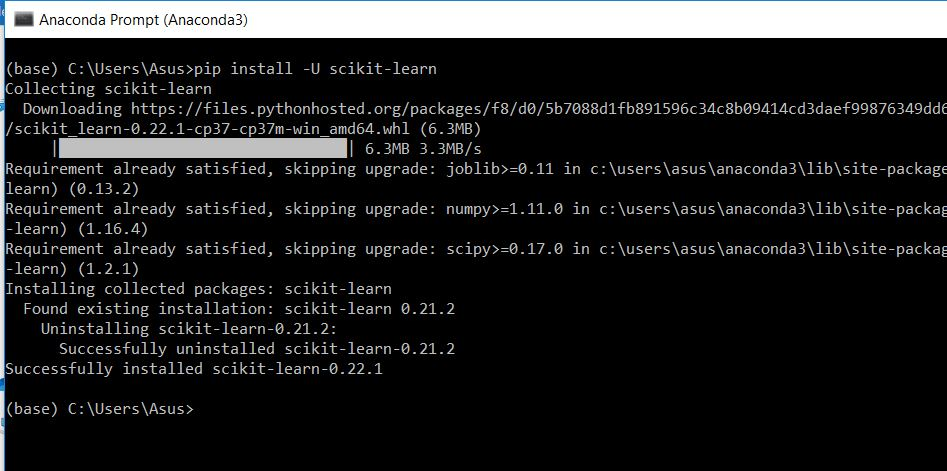
\includegraphics[width=4cm]{figures/1174034/chapter1/install1.png}
                \centering
                \caption{Instalasi}
            \end{figure}

\subsection{Percobaan}
Mencoba Library
\lstinputlisting[firstline=1, lastline=25]{src/1174034/chapter1/example1.py}
 			\begin{figure}[H]
                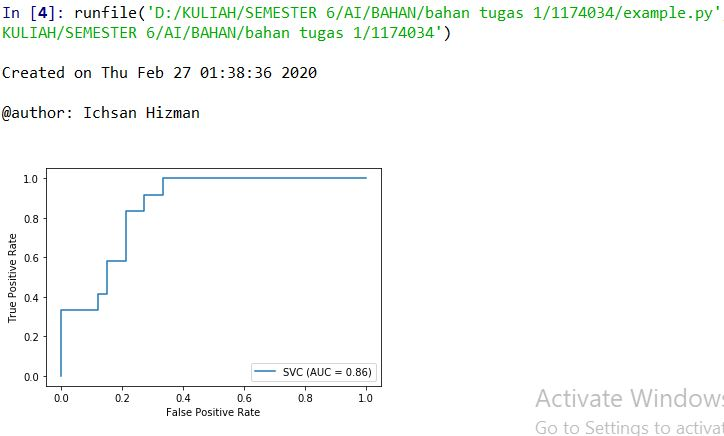
\includegraphics[width=4cm]{figures/1174034/chapter1/example1.png}
                \centering
                \caption{Variabel Explore}
            \end{figure}


\subsubsection{Mencoba Loading an example Dataset}
\lstinputlisting[firstline=1, lastline=16]{src/1174034/chapter1/datasett2.py}
		\par kemudian coba jalankan, lihat hasilnya
		\begin{figure}[H]
		\centering
		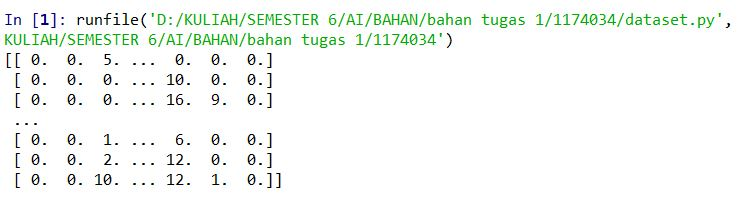
\includegraphics[width=1.5\textwidth]{figures/1174034/chapter1/dataset1.png}
		\caption{Example}
		\label{print}
		\end{figure}

\subsection{Plagiarism}
\begin{figure}[H]
\centering
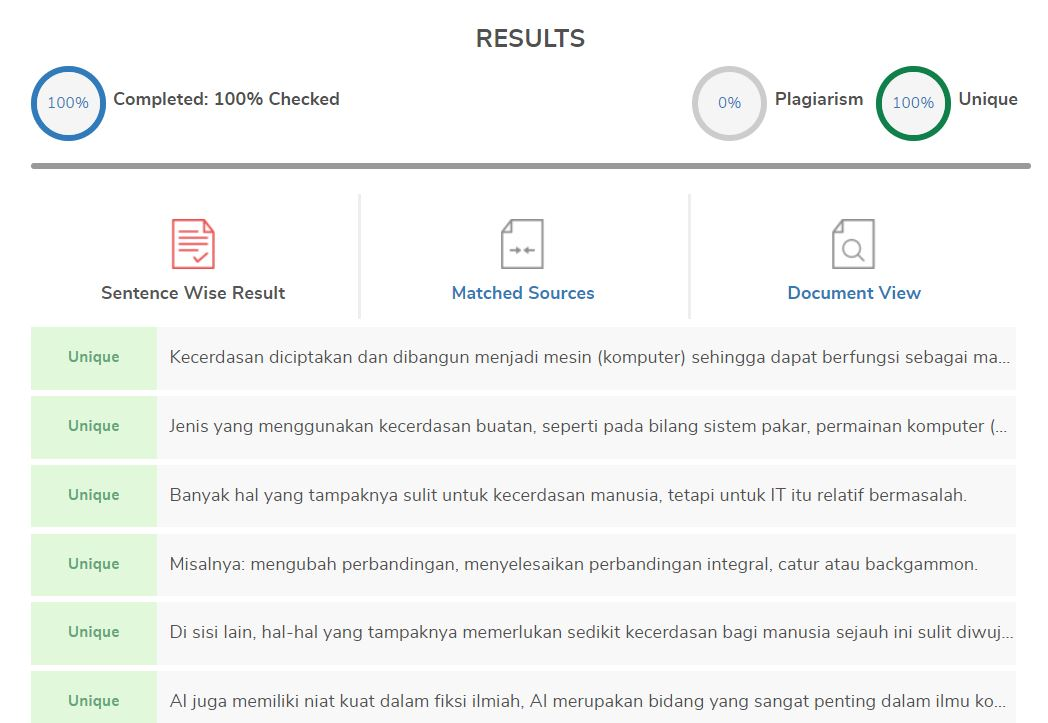
\includegraphics[scale=0.5]{figures/1174034/chapter1/plagiat1.png}
\caption{Plagiarism}
\end{figure}